%------------------------------------------------------------------------------
% This is a LaTeX template for the scientific justification of IRAM Proposals 
%------------------------------------------------------------------------------
% 
% We encourage IRAM proposers to use this template for the sake of unity 
% and clarity when Program Committee members assess their proposals.
% 
% You may customize this template to suit your preferences (e.g. using BibTex),
% but please respect the following requirements:
%     The scientific and technical justification should contain a 
%     maximum of 2 pages of text (4 pages for Large Programs), 
%     plus 2 pages of Figs., Tables and Refs.
%     The font size should be 11pt or larger.
%
% For Large Programs, the following sections should be included: 
%   i) Scientific Rationale, 
%  ii) Immediate Objective, 
% iii) Feasibility and Technical Justification, and 
%  iv) Organizational Issues.
%
%
%------------------------------------------------------------------------------
%
\documentclass[11pt,a4paper,twoside,graphicx,color]{article}
%
\usepackage[margin=2cm]{geometry}
\usepackage[margin=2cm]{geometry}
\usepackage[pdftex]{graphicx}
\usepackage{color}
\usepackage{txfonts}
\usepackage{paralist}
\usepackage[numbers]{natbib}
\setlength{\bibsep}{0.0pt}
\usepackage{amssymb}
\usepackage[breaklinks, colorlinks, citecolor=blue, linkcolor=MyBlue, urlcolor=RoyalPurple, colorlinks=true, linkcolor=blue, debug, baseurl=' ']{hyperref}
%
% Page size and text dimensions
% Do not change!
\textheight 260mm
\textwidth 178mm
\oddsidemargin -8mm
\evensidemargin -8mm
\marginparwidth 50pt
\topmargin -22mm
\brokenpenalty=10000
\sloppy
%
\bibpunct{(}{)}{;}{a}{}{,} 
\bibliographystyle{aa}
\definecolor{gris}{gray}{0.75}
%-------------------------------------------------------------------
\begin{document}
%
%
\begin{center}{\LARGE \bf
%-------------------------------------------------------------------
CO redshift search for bright NIKA distant lensed galaxy candidates
%-------------------------------------------------------------------
}\end{center}
%
\centerline{\bf P.I.: R\'emi Adam \& Alexandre Beelen}

%\paragraph{Abstract (PMS only, to be removed from here)}
%High redshift dusty star forming galaxies play a fundamental role in galaxy formation and evolution. In the quest for probing these distant objects, galaxy clusters can serve as giant telescopes, thanks to the lensing magnification they produce, to observe galaxies that would be inaccessible otherwise. We propose to use EMIR to perform the CO redshift search of two lensed dusty star forming galaxy (DSFG) candidates amplified by PSZ1 G045.85+57.71, a cluster observed with NIKA+IRAM30m. This project will allow us to obtain a detailed view on the physics of DSFGs at high redshift. We will use EMIR at the IRAM 30m telescope, primarily in the E0 band, for a total of 21.3 hours. A companion proposal was also submitted to perform the follow-up of four fainter lensed galaxy candidates, from the same initial sample, with NOEMA.

%\paragraph{Proposal history (PMS only, to be removed from here)}
%We have conducted Sunyaev-Zel'dovich (SZ) observations with the NIKA camera at the IRAM 30m telescope toward 6 clusters of galaxies in order to study the hot gas distribution in high redshift clusters and to prepare the NIKA2 SZ guaranteed time large program. Our primary goal, the mapping of the SZ effect at 150 GHz, was very successful and in addition our data have allowed us to detect sub-millimeter galaxies (in particular at 260 GHz), which are excellent high redshift lensed DSFG candidates. We therefore propose to follow-up a subset of these sources with EMIR.

%%%%%%%%%%%%%%%%%%%%%%%%%%%%%%%%%%%%%%%%%%%%%%%%
\section{Scientific context}
%========== Introduction
\paragraph{\large Introduction}
Mapping the cosmic star formation history is one of the main topics of modern cosmology, on which rapid progress has been made in the last 20 years.  We now know that star formation rate (SFR) density peaked approximately 3.5 Gyr after the Big Bang \citep{Madau2014} and declined exponentially at later times, with an e-folding timescale of 3.9 Gyr. At redshift $0.5 < z < 3$, {\bf dusty star forming galaxies} (DSFGs) are dominating the history of cosmic star formation \citep[e.g.,][]{Dole2006,Burgarella2013}. At higher $z$, we are still lacking constraints on the contribution of dusty galaxy to the star formation density.  Since optical/near-infrared observations select low dust content galaxies, observations in the (sub-)millimeter range are mandatory to target these DSFGs.

Despite the growing number of detected DSFGs at high-$z$, the detailed picture of the ongoing physical processes, which control star formation in these systems (e.g., environment, merger induced starburst, accretion of cold gas, feedback processes), is still subject to many open questions \citep{Casey2014}. This is in part due to {\bf selection effects} induced by the dust obscuration of optical light that affects the corresponding surveys, or because (sub-)millimeter wide surveys mostly capture the bright end of the luminosity function of the underlying DSFG population.

%========== Lensing to probe distant galaxies
\paragraph{\large Clusters as giant telescopes to probe distant galaxies}
The quest for high-$z$ DSFGs has been extensively addressed using large (sub-)millimeter surveys such as H-ATLAS \citep{Eales2010} or SCUBA-2 CLS \citep{Geach2016}, but they generally pick-up very luminous DSFGs that are not necessarily representative of the underlying population. A way to {\bf access more typical DSFGs is to use the lensing magnification} induced by objects on the same line of sight, such as other galaxies or {\bf galaxy clusters} \citep[e.g., SPT results,][]{Vieira2013}. In large surveys, lensed DSFGs mostly arise from galaxy-galaxy lensing, but observations in the direction of clusters, aiming at capturing cluster-galaxy lensing, present several advantages: they allow for more accurate lensing modeling (necessary to correct observables from magnification); they provide an unobscured view of the background galaxies; the involved magnification factors are generally larger; and differential magnification effects are less important.

The search for bright high-$z$ lensed DSFGs has been already used at sub-millimeter wavelength using, e.g., SCUBA \citep{Knudsen2006} or the Herschel Lensing Survey \citep[HLS,][]{Egami2010}. The discovered galaxies offer a possibility of {\bf detailed multi-wavelength observations}, in which IRAM observatories have already played an important role \citep[e.g., a $z=5.2$ galaxy behind Abell 773,][]{Combes2012}.

%========== NIKA/NIKA2 SZ LP
\paragraph{\large The NIKA \& NIKA2 cluster samples and proposed observations}
The New IRAM KIDs Arrays 2 (NIKA2) has been recently installed at the IRAM 30m telescope, offering simultaneous continuum observations at 150 and 260 GHz \citep{Catalano2016}. One of the {\bf NIKA2} guaranteed time Large Programs will consist in the observation of about {\bf 50 clusters of galaxies} in the range $0.5 < z < 1$ \citep{Comis2016}. The primary goal of this program is to image the Sunyaev-Zel'dovich (SZ) signal from the clusters' hot gas at 150 GHz. However, at these redshifts, clusters also provide {\bf optimal lenses for distant background galaxies}. Therefore, we anticipate the discovery of a large number of high-$z$ lensed DSFGs at 260 GHz around the target clusters.

As a pilot project for the NIKA2 SZ large program, we have used the {\bf prototype camera, NIKA}, to successfully map six massive clusters at $0.45 < z < 0.89$ \citep{Adam2014,Adam2015,Adam2016a,Adam2016b,Ruppin2016}. We subsequently detected several DSFGs, of which many appear to be {\bf excellent high-$z$ lensed candidates}, in particular when combining NIKA and Herschel data. Our brightest candidate \citep[lensed by \mbox{CL~J1226.9+3332} at $z=0.89$,][]{Adam2015} was also detected in HLS and has been confirmed spectroscopically as a $z$$=$$2.4$ lensed DSFG with EMIR \citep{Egami}.

Here, we propose to perform the {\bf CO redshift search} for the two brightest (and most reliable) {\bf lensed DSFG candidates} selected from one of the NIKA cluster fields, {\bf using EMIR}. As such galaxies are often too faint in optical, CO lines measurements are indeed the most efficient way to obtain spectroscopic redshifts, and in this context, EMIR is one of the most powerful instrument. Thanks to the strong magnification of our targets, we will be able to obtain a {\bf rare view on typical DSFGs at high-$z$}. In addition, the observations will be used to optimize the scientific exploitation of NIKA2 and they will allow us to open up {\bf synergies between NIKA2 and EMIR}. The cluster observations lead by our team at IRAM have been very fruitful, already resulting in 6 published/submitted papers, and this proposal is a natural continuation of this effort. A complementary companion proposal was also submitted in order to observe 4 other fainter high-$z$ DSFG candidates, from the same initial sample, with NOEMA (which are too faint for EMIR CO redshift search or have already been drawn). In particular, we aim at obtaining counterparts at other wavelength and study the connection between the optical and the sub-millimeter components (see also Table \ref{tab:candidate_summary}).

%%%%%%%%%%%%%%%%%%%%%%%%%%%%%%%%%%%%%%%%%%%%%%%%
\section{Technical justification}
%========== Sources selection
\paragraph{\large NIKA sources selection}
Four of the six NIKA clusters are part of the CLASH sample \citep{Postman2012}, for which a wealth of multi-wavelength data are publicly available, including deep HST, Spitzer, Herschel/PACS+SPIRE observations, and lensing models \citep[e.g.,][]{Zitrin2015}. The two remaining ones are {\bf Planck clusters} for which HST (3 filters, in particular to obtain the cluster mass distribution via lensing measurement, P.I. Ebeling) and SPIRE data are available. For all clusters, we have additional X-ray and SZ (NIKA) data, which we routinely use to infer the total cluster mass distribution, allowing us to validate magnification estimates.

To {\bf select lensed DSFG candidates}, we first built a source list by searching for compact objects in the highest magnification region around the clusters, in the {\bf NIKA maps}. We then searched for Herschel counterparts, focusing primarily on the long wavelength bands, but also considering shorter wavelengths (figure \ref{fig:maps}). We extracted the NIKA and Herschel fluxes of these sources, and fit the SED with a modified blackbody spectrum, as illustrated in figure \ref{fig:SED} \cite[see][for details]{Adam2016a}. A total of 17 candidates were thus found and one of the them is a known lensed DSFG at $z=2.4$, recently measured with EMIR. This procedure provides a first photometric redshift estimate assuming a typical dust temperature of $35 \pm 5$ K and propagating (nearly gaussian) fitting uncertainties. Then, we use our best fit SED together with scaling relations between the infrared (IR) luminosity  and the CO line intensity \citep{Greve2014} to compute the expected CO(3-2) and CO(4-3) signal in EMIR E0 band. These lines are the most likely to be observed according to our redshift estimates \citep{Carilli2013}, but the estimates remains comparable for other J lines. The source list and their main properties are given in Table \ref{tab:candidate_summary}. The two brightest candidates (in terms of CO line flux) with sufficiently well constrained SED (i.e., with the most accurate flux predictions), excluding SMG01 (already observed with EMIR), are SMG11 and SMG12 in the {\bf field of \mbox{PSZ1G045.85+57.71}}. We therefore propose to observe these {\bf two sources} (see figure \ref{fig:maps}).

%========== Immediate objectives
\paragraph{\large Immediate objectives}
The proposed observations will allow us to fulfill the following immediate objectives. {\bf 1)} We will obtain {\bf spectroscopic redshifts} for the two NIKA discovered distant DSFGs. This will provide a direct confirmation that our candidates are indeed high-$z$ objects. {\bf 2)} The knowledge of the redshift will allow us to convert primary observables to physically relevant quantities, in order to characterize the {\bf galaxy properties (SFR, IR luminosity, etc)}. {\bf 3)} We will estimate the amount of {\bf molecular gas} of each galaxy and it will be compared to the {\bf amount of dust} probed by continuum photometric data. {\bf 4)} Using the line profiles, we will search for {\bf evidence of merging}, that may drive {\bf starburst activity}. {\bf 5)} Finally, such observations will demonstrate the strong synergies between NIKA2 and EMIR observations.

%========== Time and configuration
\paragraph{\large Time estimates and configuration strategy}
Only three separate tuning are necessary to {\bf cover the entire E0 band} from 73 to 117 GHz, with 16 GHz bandwidth. This corresponds to redshifts between 1.0 and 8.7 for CO lines between $J=2-1$ and $7-6$, with only a small gap at $1.78 < z < 1.98$ that is very unlikely for our targets based on the photometric redshift estimates of Table \ref{tab:candidate_summary}. We propose to start the search in the lowest frequency band (using the tracked WSW observing mode) because of the better atmospheric conditions and the access to the lower J CO lines, the higher being possibly weaker. Once the first line is observed, we will search for a second one in the E1 band.

We consider the CO(3-2) and CO(4-3) lines because they are the most likely to be found in the E0 band at the expected redshift (4.6 and 3.6 for SMG11 and SMG12), but our estimates remain comparable for other J lines. For these two lines, we expect the flux to be, respectively, about 31 and 19 mJy for SMG11, and about 25 and 15 mJy for SMG12 (Table \ref{tab:candidate_summary}). We aim at a $5 \sigma$ detection of the lines, which correspond for CO(3-2) and CO(4-3), respectively, to a rms of 1.05 and 0.63 mK for SMG11 and 0.84 and 0.51 mK for SMG12. We need a {\bf resolution of 80 km/s} to ensure a good line sampling. Therefore, including 50\% overhead for calibration, assuming a typical elevation of 50 degrees and average winter conditions (4.0 mm of pwv, Tsys 122.8 K[Ta*] mean per pixel), we require 2.6 hours and 3.5 hours of telescope time per tuning for SMG11 and SMG12 respectively, according to the EMIR time estimator. We allow 3 tunings in order to cover the full E0 band, and we add 30 min per tuning. Therefore, the total telescope time required to search for CO lines toward SMG11 and SMG12 are {\bf 9.3 hours and 12 hours, i.e., a total of 21.3 hours}. Finally, the two sources are observable $\sim 10$ hours per day during the winter semester.

%%%%%%%%%%%%%%%%%%%%%%%%%%%%%%%%%%%%%%%%%%%%%%%%
\newpage
\section{Supporting material}
%========== Multi-lambda figure
\begin{figure}[h!]
	\centering
	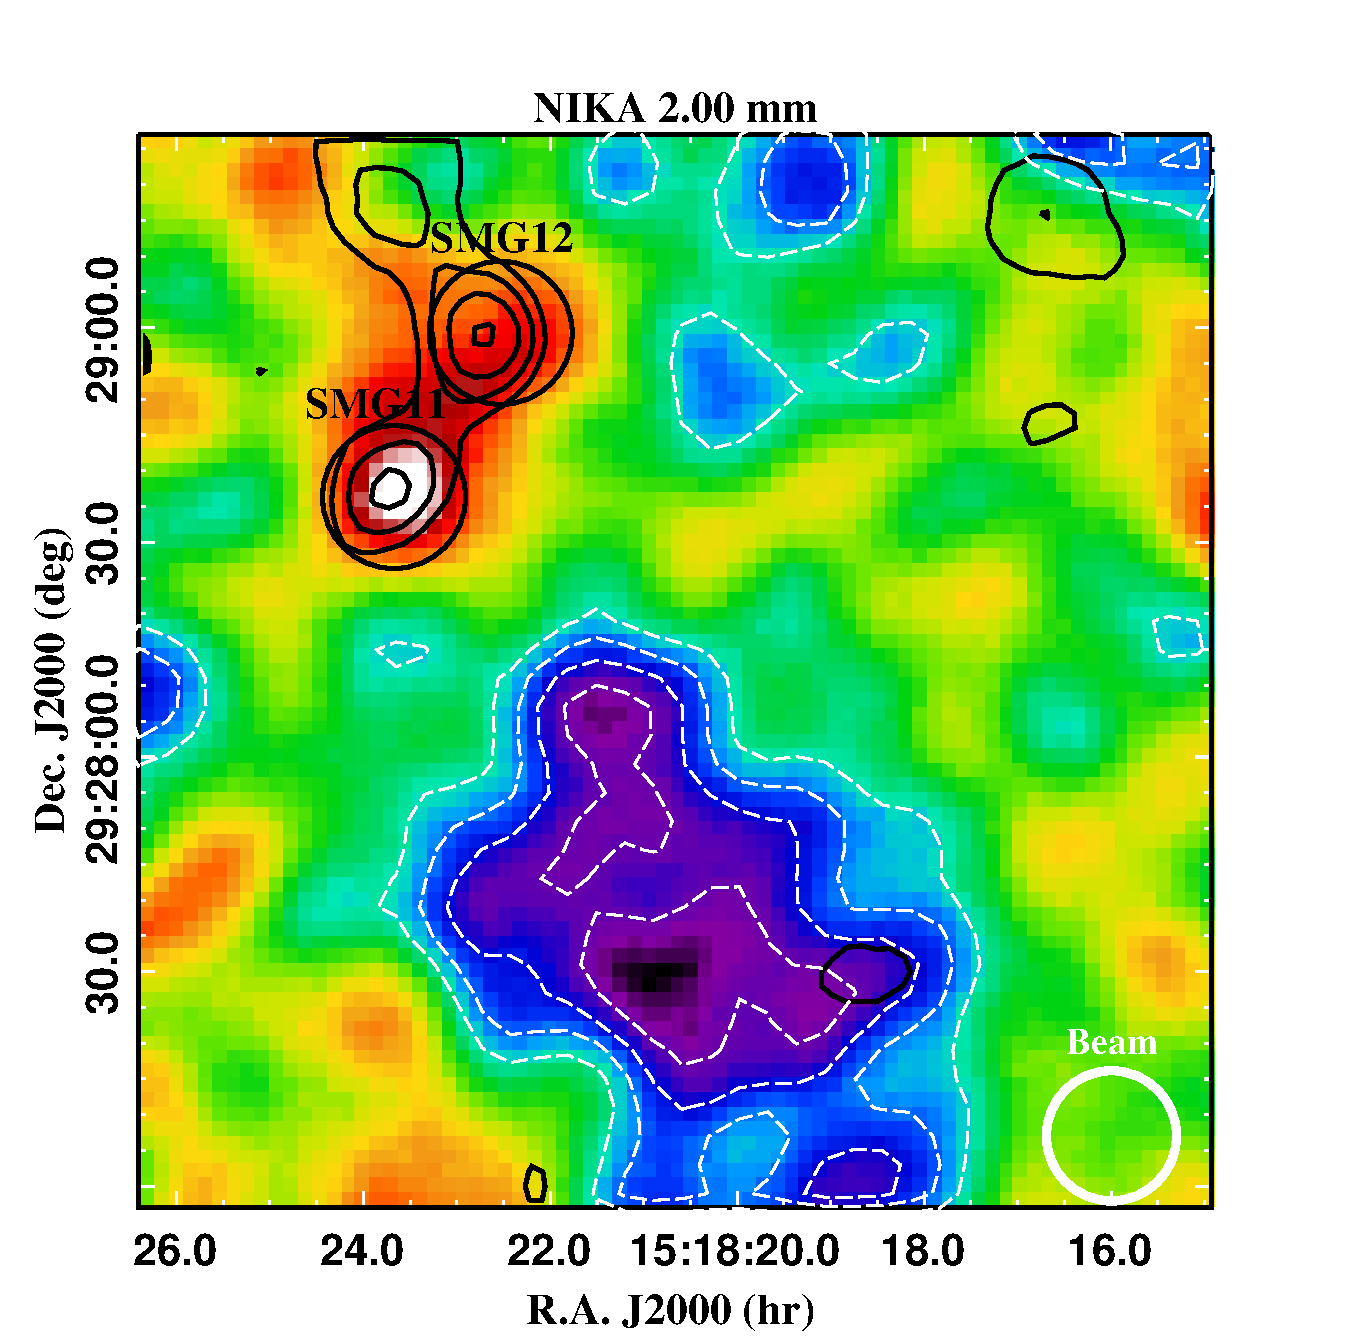
\includegraphics[width=0.49\textwidth]{MultiL_PSZ1G045_2mm.pdf}
	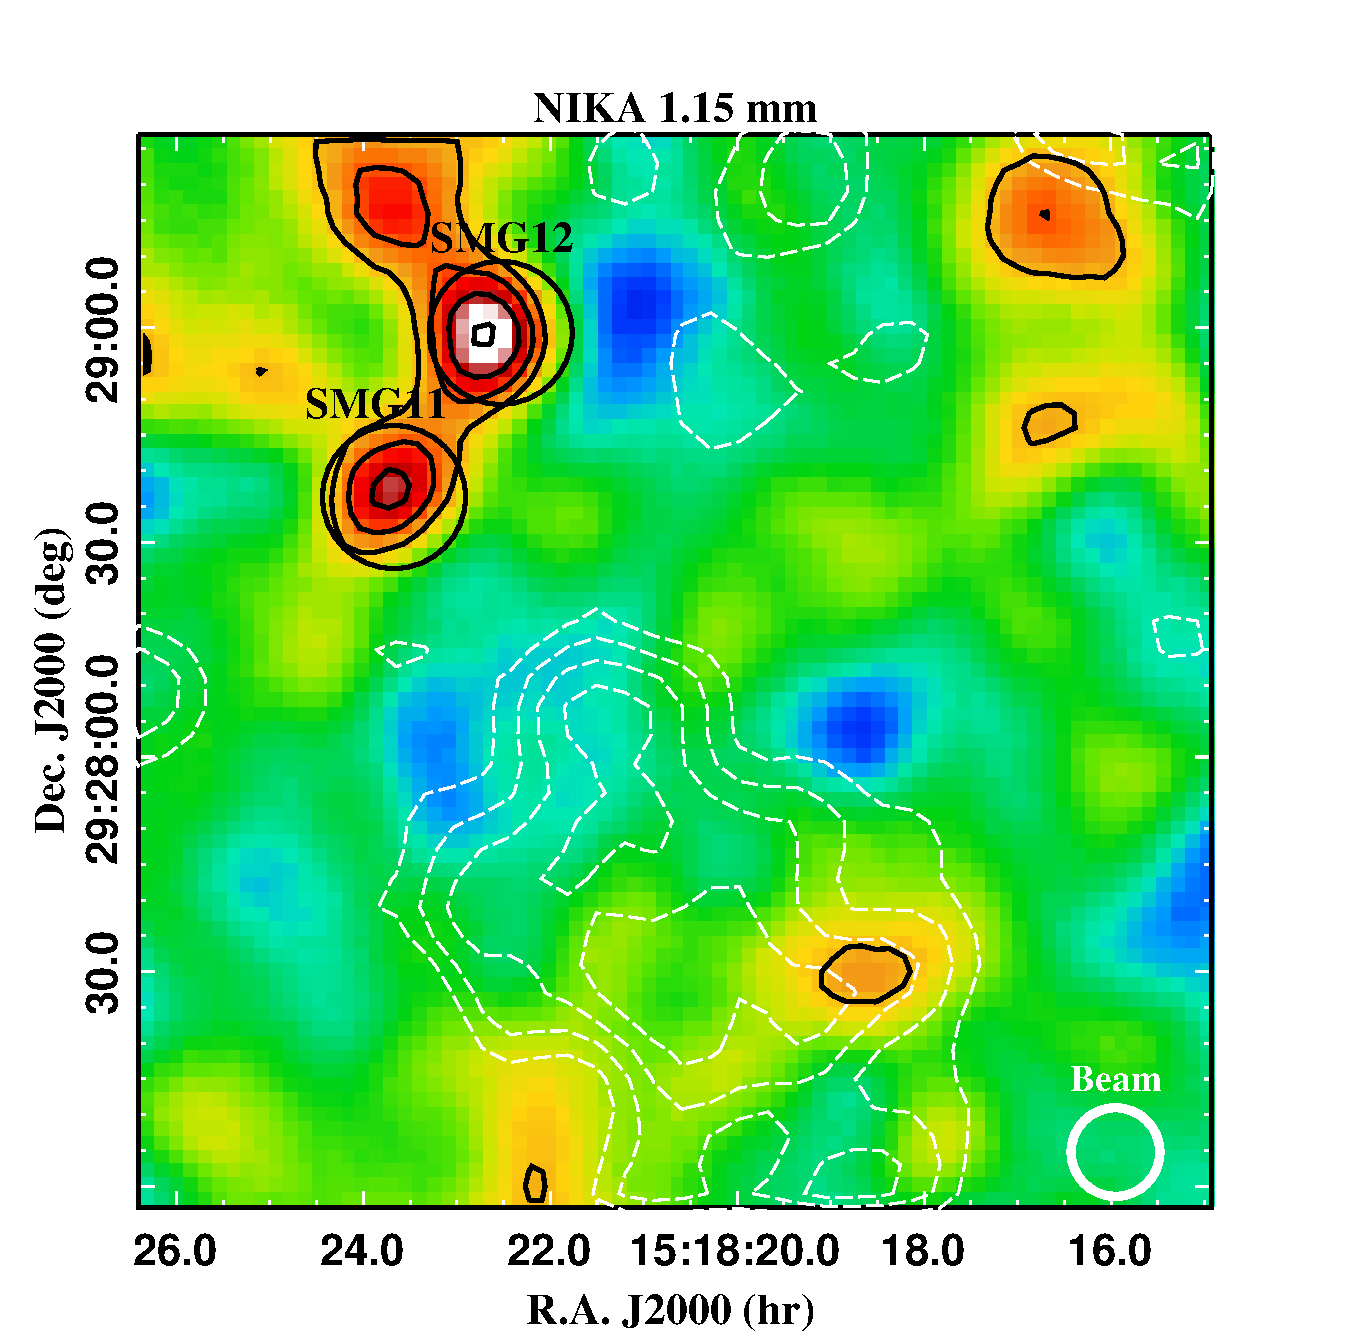
\includegraphics[width=0.49\textwidth]{MultiL_PSZ1G045_1mm.pdf}
	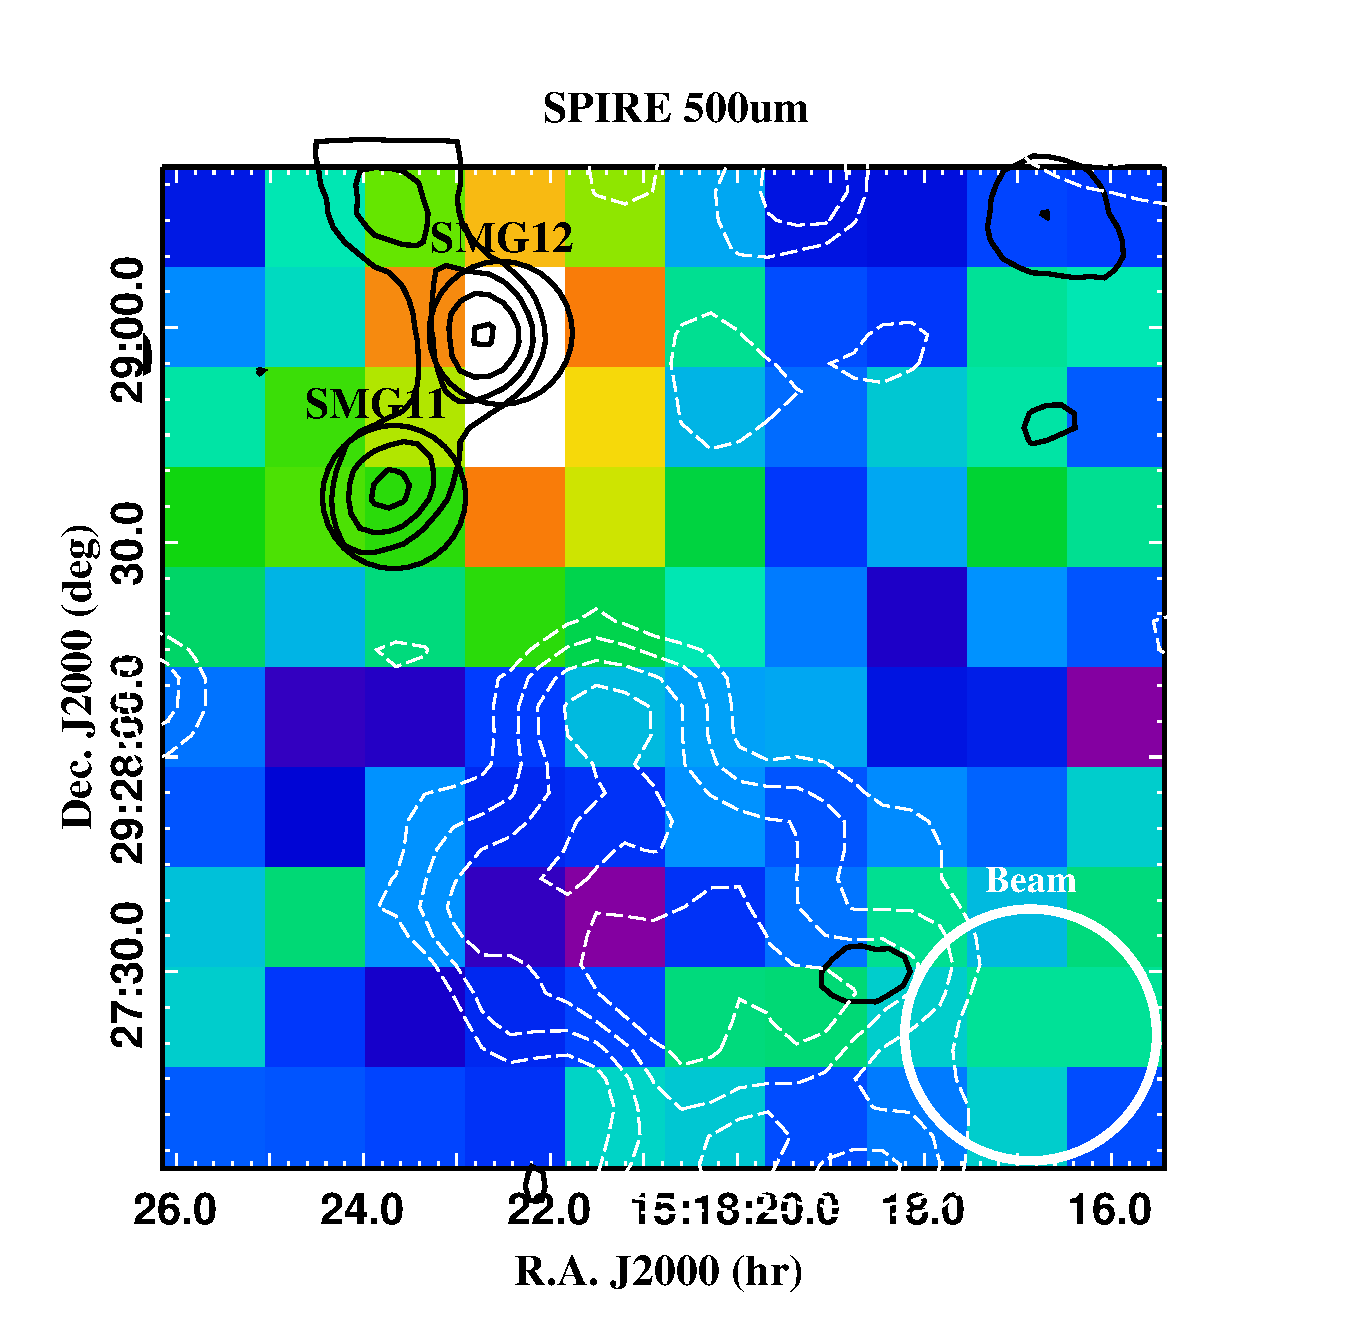
\includegraphics[width=0.33\textwidth]{MultiL_PSZ1G045_500.pdf}
	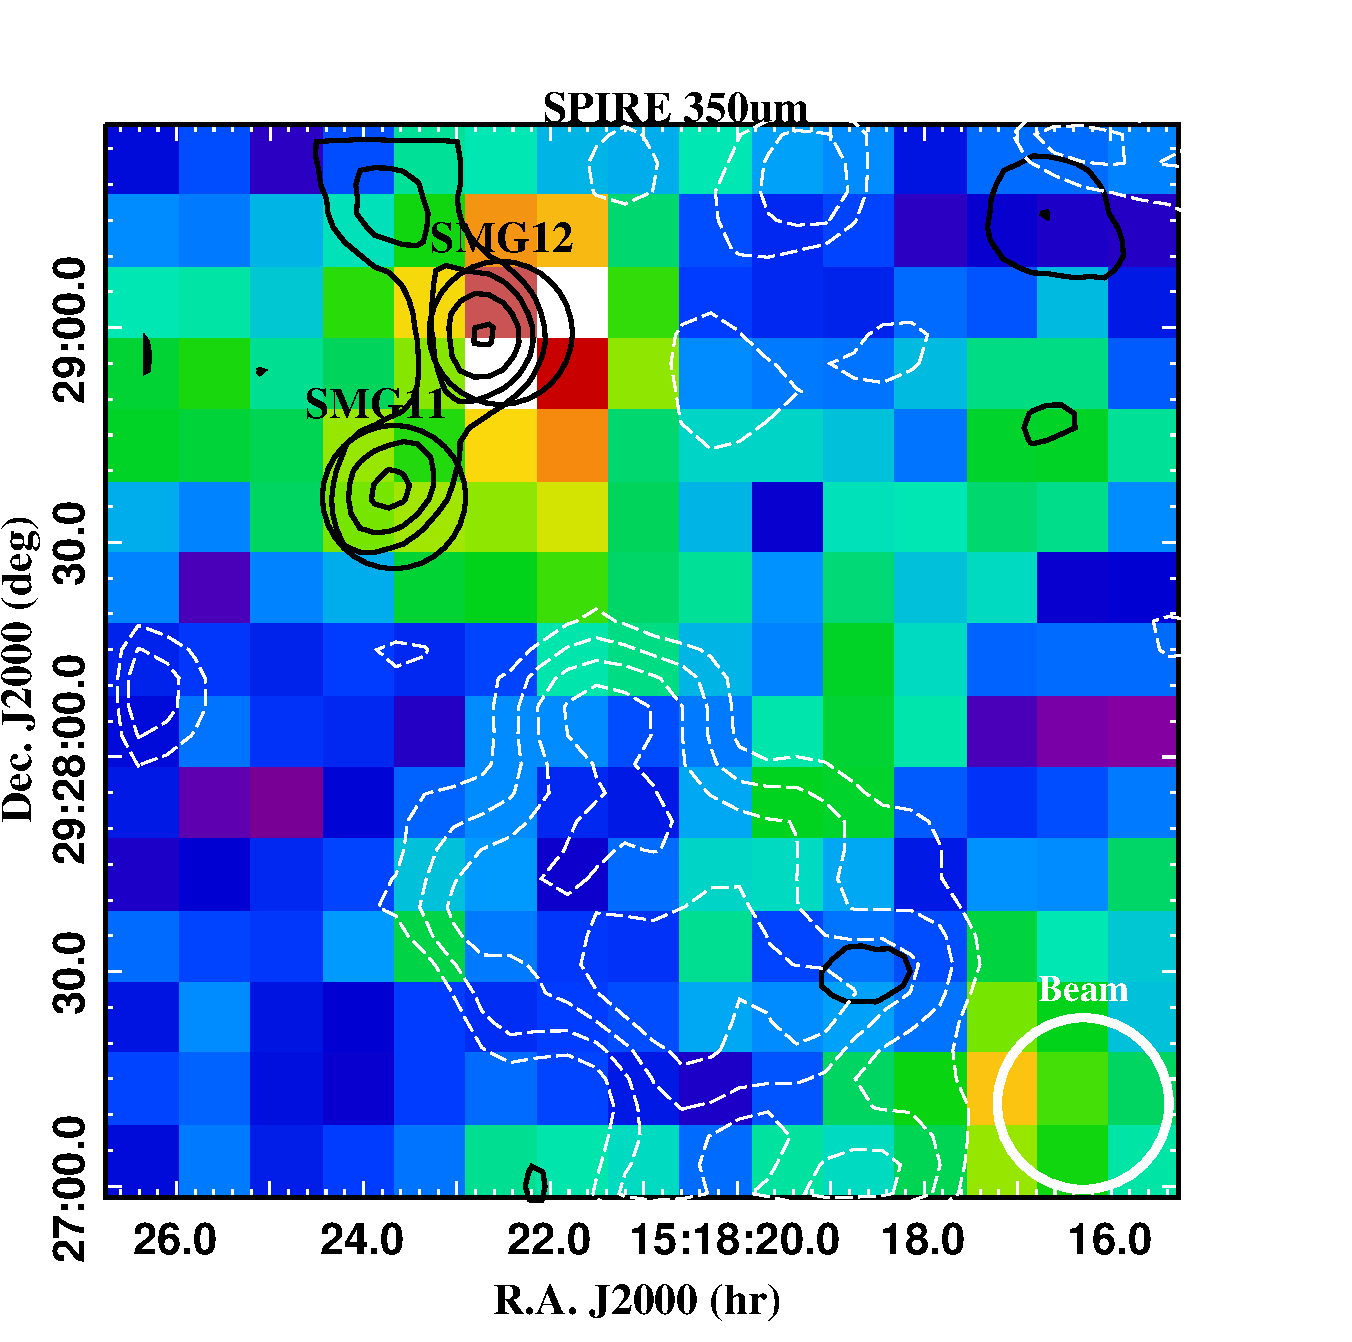
\includegraphics[width=0.33\textwidth]{MultiL_PSZ1G045_350.pdf}
	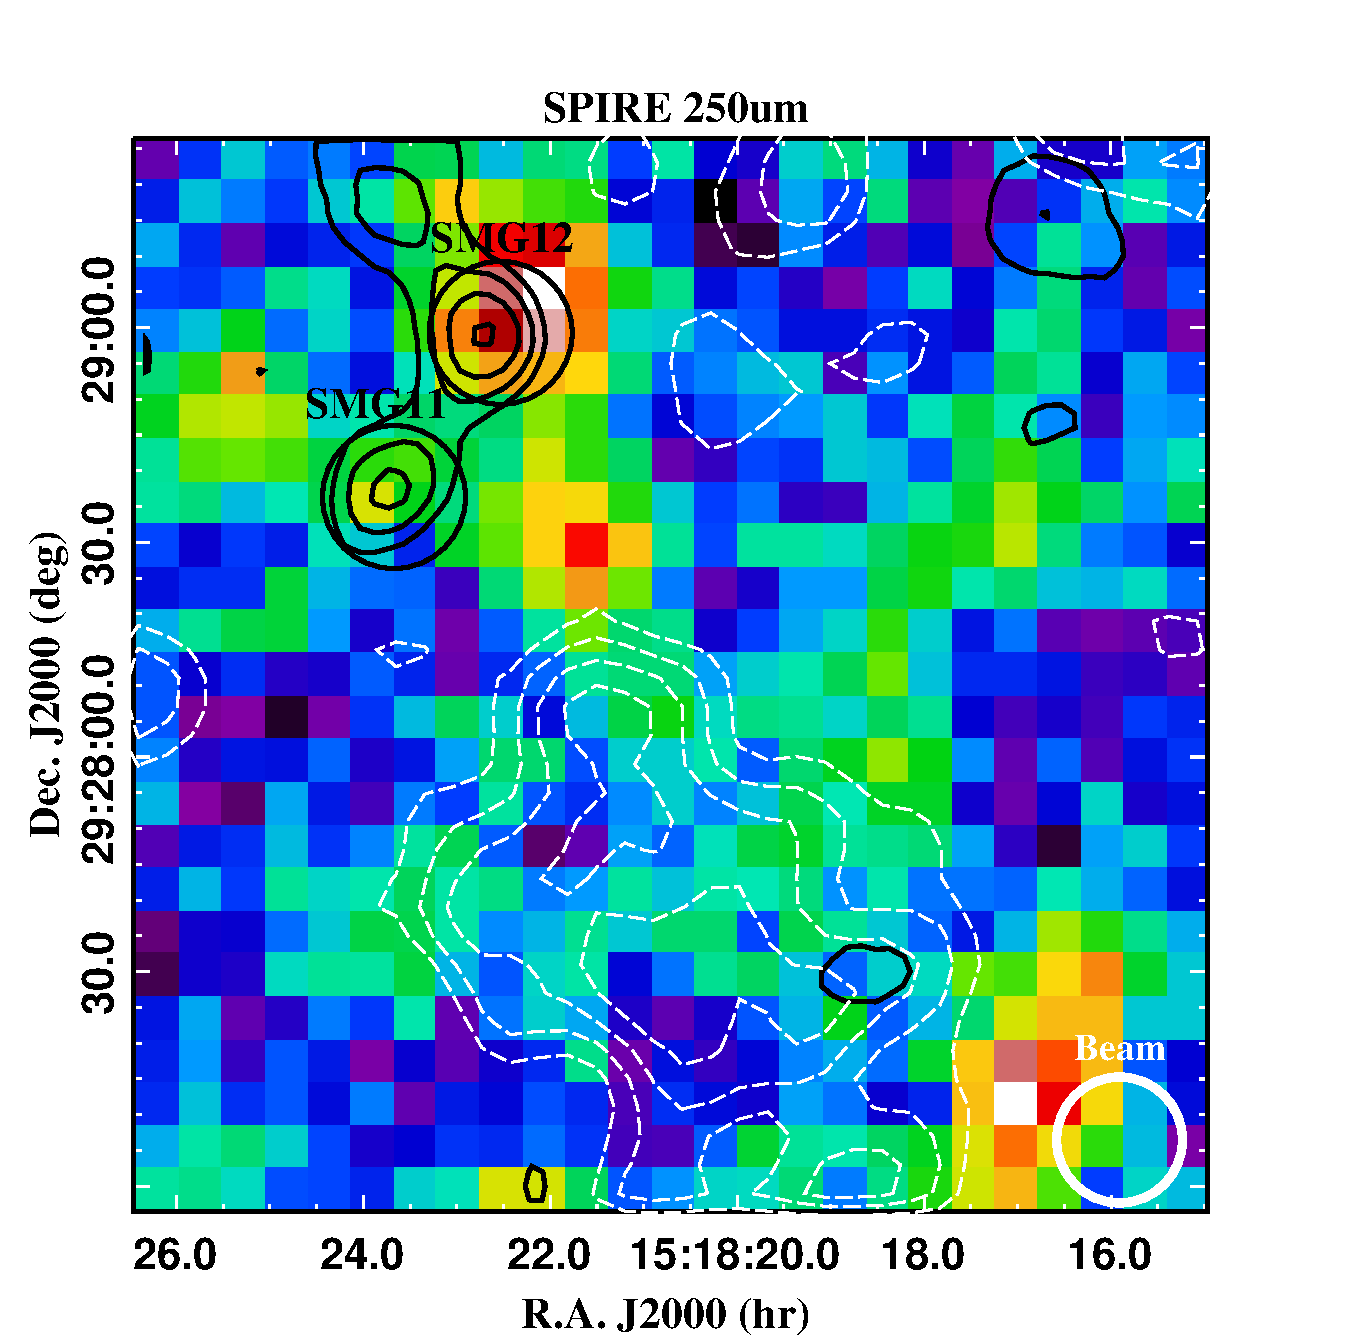
\includegraphics[width=0.33\textwidth]{MultiL_PSZ1G045_250.pdf}
	\caption{\footnotesize{Millimeter (top) and sub-millimeter (bottom) maps toward \mbox{PSZ1~G045.9+57.7}. From top to bottom and left to right, the channels are NIKA 2.00 and 1.15 mm, and SPIRE 500, 350 and 250 $\mu$m. Black contours are reproduced from the 1.15 mm map to highlight the two bright DSFG candidates. The two candidates, labeled on the figure, are also identified by black circles. The elongated negative signal at 2.00 mm is due to SZ signal \citep{Ruppin2016} and the white dashed contours are reproduced from this map to highlight the cluster mass distribution location. The white circles on the bottom right of each map provide the beam FWHM of each channel.}}
	\label{fig:maps} 
\end{figure}

%========== SED figure
\begin{figure}[h!]
	\centering
	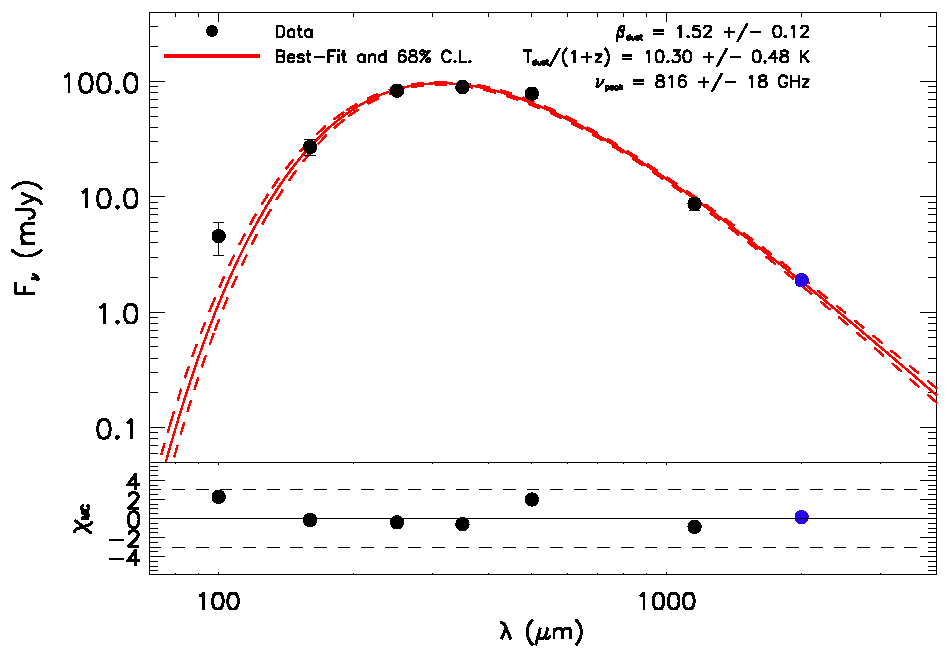
\includegraphics[trim=0cm 0cm 0.18cm 0cm, clip=true, height=4.55cm]{SED_fit01.pdf}
	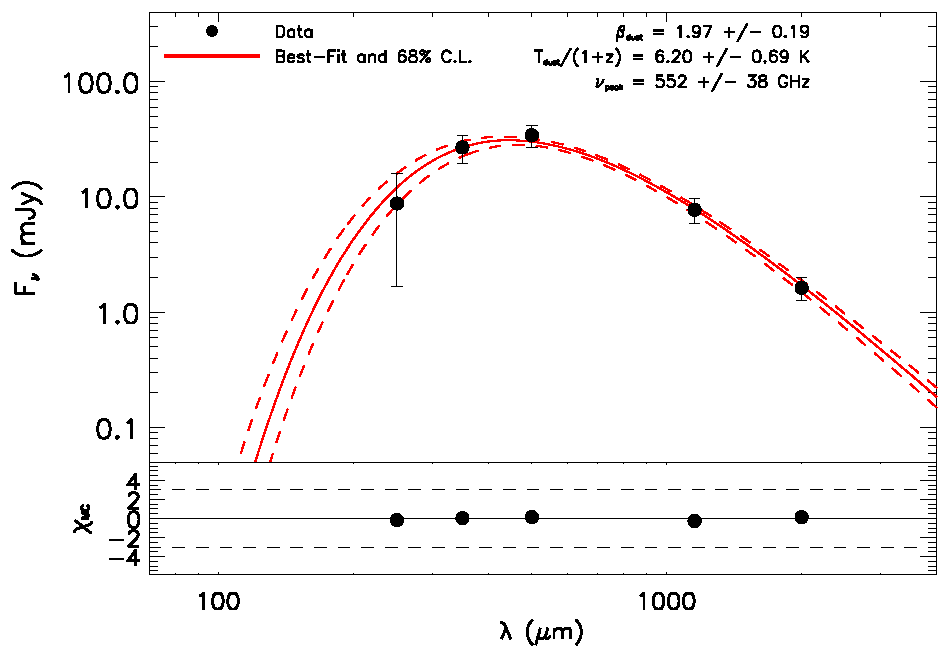
\includegraphics[trim=2.5cm 0cm 0.18cm 0cm, clip=true, height=4.55cm]{SED_fit11.pdf}
	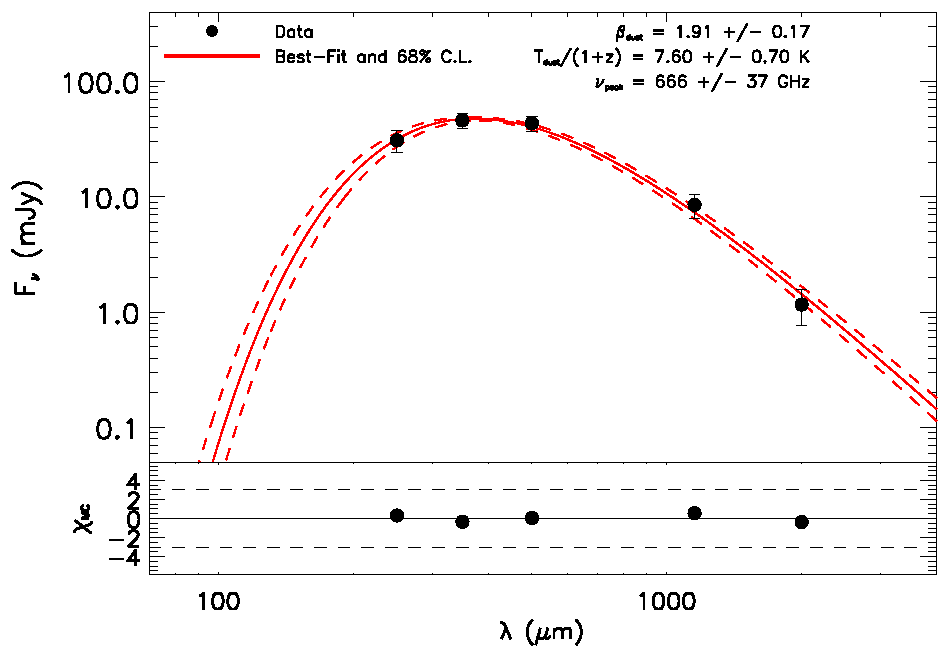
\includegraphics[trim=2.5cm 0cm 0cm 0cm, clip=true, height=4.55cm]{SED_fit12.pdf}
	\caption{\footnotesize{NIKA+Herschel SED and their modified black-body fit constraint. The blue point indicates possible contamination from SZ signal. {\bf Left:} SMG01 (lensed by \mbox{CL~J1226.9+3332}) -- bright lensed DSFG with confirmed redshift at $z = 2.4$ from EMIR observations. Our redshift estimates gives $\hat{z} = 2.4 \pm 0.5$ for this source. This SED is provided as a reference for comparison. {\bf Middle and right:} SMG11 and SMG12, respectively (lensed by \mbox{PSZ1~G045.85+57.71}) -- high redshift candidates with $>3 \sigma$ NIKA detection in the two bands. Our redshift estimates gives $\hat{z} = 4.6 \pm 1.0$ and $\hat{z} = 3.6 \pm 0.8$ for SMG11 and SMG12, respectively. See also Figure \ref{fig:maps}.}}
	\label{fig:SED} 
\end{figure}

%========== Table of candidates
\begin{table}[h]
\caption{\footnotesize{Summary of the properties of the lensed DSFG candidates. The 2 sources selected for the proposed observations are in bold face. The four sources proposed for NOEMA observations, in order to complement this proposal, are marked by $^{\dagger}$. Note that the physical quantities are not corrected for magnification to provide the direct observables. The CO line fluxes assume that the line widths are 400 km/s.}}
\begin{center}
\resizebox{\columnwidth}{!} {
\begin{tabular}{c|cccc|ccccccccc}
\hline
\hline
Source & R.A. & Dec. & 1.15 mm flux & 2.00 mm flux & SED peak & $\beta_{\rm dust}$ & $T_{\rm eff,dust}$ & $\hat{z}_{\rm phot}$ & $\hat{L}_{\rm IR}$ & $\hat{\rm SFR}$ & $\hat{F}_{\rm CO(3-2)}$ & $\hat{F}_{\rm CO(4-3)}$ & \\
 & (degree) & (degree) & (mJy) & (mJy) & (GHz) & ( --- ) & (K) & ( --- ) & ($10^{12}$ L$_{\odot}$) & (M$_{\odot}$ / yr) & (mJy) & (mJy) \\
\hline
RXJ1347.5-1145 & \multicolumn{13}{c}{--- no strong candidate ---} \\
\hline
CLJ1226.9+3332 SMG01$^{\dagger}$ & 186.74940 & 33.543114 & $8.7 \pm 1.1$ & $1.9 \pm 0.2$$^{*}$ & $816 \pm 18$ & $1.52 \pm 0.12$ & $10.3 \pm 0.5$ & $2.4 \pm 0.5$ & $48.0$ & $8202.0$ & $18.7$ & $11.8$ \\
CLJ1226.9+3332 SMG02$^{\dagger}$ & 186.75814 & 33.549083 & $3.1 \pm 1.1$ & $0.9 \pm 0.3$$^{*}$ & $609 \pm 66$ & $2.05 \pm 0.19$ & $6.7 \pm 1.0$ & $4.2 \pm 1.1$ & $45.1$ & $7706.3$ & $16.5$ & $10.4$ \\
\hline
MACSJ1423.8+2404 SMG03 & 215.94946 & 24.070625 & $8.6 \pm 2.5$ & $-0.4 \pm 0.5$$^{**}$ & $911 \pm 88$ & $0.89 \pm 0.20$ & $14.0 \pm 1.2$ & $1.5 \pm 0.4$ & $3.7$ & $641.2$ & $1.8$ & $1.4$ \\
MACSJ1423.8+2404 SMG04 & 215.93582 & 24.054733 & $4.6 \pm 2.7$ & $-0.3 \pm 0.6$ & $608 \pm 792$ & $2.17 \pm 0.20$ & $6.5 \pm 10.0$ & $4.4 \pm 8.2$ & $32.0$ & $5480.4$ & $11.7$ & $7.6$ \\
MACSJ1423.8+2404 SMG05 & 215.94742 & 24.080956 & $4.2 \pm 2.4$ & $-0.8 \pm 0.5$$^{**}$ & $751 \pm 142$ & $1.00 \pm 0.19$ & $11.1 \pm 1.8$ & $2.2 \pm 0.7$ & $5.7$ & $971.5$ & $2.3$ & $1.7$ \\
MACSJ1423.8+2404 SMG06 & 215.97167 & 24.062847 & $7.6 \pm 2.7$ & $0.8 \pm 0.6$ & $359 \pm 1530$ & $2.05 \pm 0.20$ & $4.0 \pm 18.9$ & $7.8 \pm 42.2$ & $61.2$ & $10472.3$ & $25.7$ & $15.8$ \\
\hline
MACSJ0717.5+3745 SMG07$^{\dagger}$ & 109.37740 & 37.745272 & $2.5 \pm 0.7$ & $0.6 \pm 0.2$$^{*}$ & $424 \pm 103$ & $1.86 \pm 0.19$ & $4.9 \pm 1.4$ & $6.1 \pm 2.3$ & $25.9$ & $4431.6$ & $10.1$ & $6.6$ \\
MACSJ0717.5+3745 SMG08 & 109.38925 & 37.734656 & $1.5 \pm 0.7$ & $-0.1 \pm 0.2$$^{*}$ & $731 \pm 1615$ & $2.10 \pm 0.20$ & $8.0 \pm 20.0$ & $3.4 \pm 11.1$ & $11.8$ & $2014.6$ & $4.3$ & $3.0$ \\
MACSJ0717.5+3745 SMG09$^{\dagger}$ & 109.39919 & 37.759447 & $1.7 \pm 0.7$ & $0.2 \pm 0.2$$^{*}$ & $653 \pm 150$ & $2.38 \pm 0.20$ & $6.7 \pm 2.0$ & $4.2 \pm 1.7$ & $27.0$ & $4610.0$ & $9.9$ & $6.5$ \\
MACSJ0717.5+3745 SMG10 & 109.35268 & 37.726572 & $1.4 \pm 0.9$ & $0.1 \pm 0.2$ & $865 \pm 112$ & $2.29 \pm 0.19$ & $9.0 \pm 1.5$ & $2.9 \pm 0.9$ & $18.8$ & $3211.5$ & $7.0$ & $4.7$ \\
\hline
{\bf PSZ1G045.85+57.71 SMG11} & 229.59864 & 29.476758 & $7.7 \pm 1.9$ & $1.6 \pm 0.4$ & $552 \pm 38$ & $1.97 \pm 0.19$ & $6.2 \pm 0.7$ & $4.6 \pm 1.0$ & $84.2$ & $14392.5$ & $31.0$ & $18.7$ \\
{\bf PSZ1G045.85+57.71 SMG12} & 229.59388 & 29.483133 & $8.5 \pm 2.0$ & $1.2 \pm 0.4$ & $666 \pm 37$ & $1.91 \pm 0.17$ & $7.6 \pm 0.7$ & $3.6 \pm 0.8$ & $67.9$ & $11615.2$ & $24.8$ & $15.2$ \\
PSZ1G045.85+57.71 SMG13 & 229.57727 & 29.458097 & $4.5 \pm 1.7$ & $-0.8 \pm 0.3$$^{**}$ & $389 \pm 1570$ & $2.06 \pm 0.20$ & $4.3 \pm 19.3$ & $7.2 \pm 36.7$ & $57.6$ & $9854.6$ & $23.4$ & $14.5$ \\
PSZ1G045.85+57.71 SMG14 & 229.59208 & 29.447528 & $3.4 \pm 1.7$ & $0.3 \pm 0.3$$^{*}$ & $801 \pm 1506$ & $0.92 \pm 0.20$ & $12.2 \pm 18.8$ & $1.9 \pm 4.5$ & $3.2$ & $545.1$ & $1.4$ & $1.1$ \\
\hline
PSZ1G046.13+30.75 SMG15 & 259.28271 & 24.041972 & $3.5 \pm 3.0$ & $1.2 \pm 0.5$ & $635 \pm 811$ & $1.05 \pm 0.21$ & $9.2 \pm 10.3$ & $2.8 \pm 4.2$ & $11.6$ & $1975.9$ & $4.3$ & $3.0$ \\
PSZ1G046.13+30.75 SMG16 & 259.26292 & 24.062750 & $-1.2 \pm 2.4$ & $1.0 \pm 0.4$$^{*}$ & $762 \pm 333$ & $1.07 \pm 0.20$ & $11.0 \pm 4.3$ & $2.2 \pm 1.3$ & $7.7$ & $1321.8$ & $3.1$ & $2.2$ \\
PSZ1G046.13+30.75 SMG17 & 259.28542 & 24.074583 & $0.0 \pm 2.3$ & $1.1 \pm 0.4$$^{*}$ & $716 \pm 860$ & $0.92 \pm 0.21$ & $10.9 \pm 10.7$ & $2.2 \pm 3.2$ & $6.0$ & $1024.2$ & $2.4$ & $1.8$ \\
\hline
\end{tabular}
}
\end{center}
{\small {\bf Notes.} $^{*}$ Possibly contaminated by SZ signal. $^{**}$ Very likely to be contaminated by SZ signal.}
\label{tab:candidate_summary}
\end{table}

%%%%%%%%%%%%%%%%%%%%%%%%%%%%%%%%%%%%%%%%%%%%%%%%
\begin{thebibliography}{9}
{\scriptsize

\bibitem[Adam et al.(2014)]{Adam2014}
R. Adam, B. Comis, J.~F. Mac\'ias-P\'erez, et al. (2014), A\&A, 569, A66, ArXiv:1310.6237

\bibitem[Adam et al.(2015)]{Adam2015}
R. Adam, B. Comis, J.~F. Mac\'ias-P\'erez, et al. (2015), A\&A, 576, A12, ArXiv:1410.2808

\bibitem[Adam et al.(2016a)]{Adam2016a}
R. Adam, B. Comis, I. Bartalucci, et al. (2016), A\&A, 586, A122, ArXiv:1510.06674

\bibitem[Adam et al.(2016b)]{Adam2016b}
R. Adam, I. Bartalucci, G.~W. Pratt, et al. (2016), A\&A, submitted, ArXiv:1606.07721

\bibitem[Burgarella et al.(2013)]{Burgarella2013}
D. Burgarella, V. Buat, C. Gruppioni, et al. (2013), A\&A, 554, A70, ArXiv:1304.7000
	
\bibitem[Casey et al.(2014)]{Casey2014}
C.-M. Casey, D. Narayanan, \& A. Cooray (2014), Phys. Rep., 541, 45, ArXiv:1402.1456

\bibitem[Carilli \& Walter(2013)]{Carilli2013}
C. L. Carilli \& F. Walter 2013, ARAA, 51, 105, ArXiv:1301.0371

\bibitem[Catalano et al.(2016)]{Catalano2016}
A. Catalano, R. Adam, P. Ade, et al. (2016), ArXiv:1605.08628

\bibitem[Combes et al.(2012)]{Combes2012}
F. Combes, M. Rex, T.~D. Rawle, et al. (2012), A\&A, 538, L4, ArXiv:1201.2908

\bibitem[Comis et al.(2016)]{Comis2016}
B. Comis, R. Adam, P. Ade, et al. (2016), Moriond Proceeding, ArXiv:1605.09549

\bibitem[Dole et al.(2006)]{Dole2006}
H. Dole, G. Lagache, J.-L. Puget, et al. (2006), A\&A, 451, 417, ArXiv:0603208

\bibitem[Geach et al.(2016)]{Geach2016}
J. E. Geach, J. S. Dunlop, M. Halpern et al. (2016), MNRAS, submitted, ArXiv:1607.03904

\bibitem[Eales et al.(2010)]{Eales2010}
S. Eales, L. Dunne, D. Clements, et al. (2010), PASP, 122, 499, ArXiv:0910.4279

\bibitem[Egami et al.(2010)]{Egami2010}
E. Egami, M. Rex, T.~D.. Rawle, et al. (2010), A\&A, 518, L12, ArXiv:1005.3820

\bibitem[Egami(priv. com.)]{Egami}
E. Egami, private communication

\bibitem[Greve et al.(2014)]{Greve2014}
T. R. Greve, I. Leonidaki, E. M. Xilouris, et al. 2014, ApJ, 794, 142, ArXiv:1407.4400

\bibitem[Knudsen et al.(2006)]{Knudsen2006}
K. K. Knudsen, V. E. Barnard, P. P. van der Werf, et al. 2006, MNRAS, 368, 487, ArXiv:0602131

\bibitem[Madau \& Dickinson (2014)]{Madau2014}
P. Madau \& M. Dickinson 2014, A\&ARA, 52, 415, ArXiv:1403.0007

\bibitem[Postman et al.(2012)]{Postman2012}
M. Postman, D. Coe, N. Ben\'itez, et al. 2012, ApJS, 199, 25, ArXiv:1106.3328

\bibitem[Ruppin et al.(2016)]{Ruppin2016}
F. Ruppin, R. Adam, B. Comis, et al. 2016, A\&A, submitted, ArXiv:1607.07679

\bibitem[Vieira et al.(2013)]{Vieira2013}
J.~D. Vieira, D.~P. Marrone, S.~C. Chapman, et al. 2013, Nature, 495, 344, ArXiv:1303.2723

\bibitem[Zitrin et al.(2015)]{Zitrin2015}
A. Zitrin, A. Fabris, J. Merten, et al. 2015, ApJ, 801, 44, ArXiv:1411.1414

}
\end{thebibliography}

\end{document}
